\chapter{Methodology and Experiment Setup}\label{ch:Methods}
In this chapter the methods used to collect the data is provided along with
justifications. This study required the execution of several IPD tournaments and
thus appropriate software needed to be implemented and tested for accuracy. All
the appropriate code, written for this project, is made available in the GitHub
repository (https://github.com/shapperzsm/final-project).

\section{Data Collection Algorithm}\label{sec:Data_Collection_Algorithm}
This section describes the overall algorithm used to obtain the data and the
attributes collected. Firstly, the aim of this exercise was
to illustrate the Folk Theorem and analyse the \(p\)-thresholds via a large
experiment. It was expected that plots similar to Figure~\ref{fig:flk_thm_plt}
would be yielded. This clearly shows that there eventually exists a
\(p_{e}\) where defection is not a rational decision.

\begin{figure}
    \centering
    % Example plot
\begin{tikzpicture}
    \draw[->] (0,0) -- (5.5,0) node[right]{$p_{e}$};
    \draw[->] (0,0) -- (0,5.5) node[above]{$min{\{p_{d}\}}$};
    \draw[red, very thick] (0,0) -- (2,0);
    \draw[red, very thick] (2,0) -- (2,5);
    \draw[red, very thick] (2,5) -- (5, 5);
    \draw[blue, dashed, very thick] (2,-0.5) -- (2,5.5);
    \node[blue] at (4, 3) {$p$-threshold};
    \node[below] at (0,0) {0};
    \node[below] at (5,0) {1};
    \node[left] at (0,5) {1};
    \draw[->, thin] (3.5, 2.75) -- (2.25,0.25);
\end{tikzpicture}
    \caption{An example plot illustrating the \(p\)-threshold as indicated by the Folk Theorem. The minimum probability of defection in equilibria is denoted \(\min \{p_{d}\} \).}\label{fig:flk_thm_plt}
\end{figure}

Therefore, to observe whether any environmental settings of the
tournament do affect the p-threshold, a large amount of data was needed. This
was in order for any observations made to be statistically significant. Figure~\ref{fig:alg_diag} shows
a pictorial representation of the collection method used. Each step visible is
explained in detail throughout this chapter with further references to
appropriate sections.

\begin{figure}
    \centering
    \resizebox{\textwidth}{!}{% Algorithm Diagram
\begin{tikzpicture}[roundnode/.style={circle, draw=green!60, fill=green!5, very
thick, minimum size=7mm}, squarenode/.style={rectangle, draw=red!60, fill=red!5,
very thick, minimum size=5mm},
]
    \node[squarenode](start) {START};
    \node[roundnode](database) [right=of start] {\begin{tikzpicture}
    \draw[thin] (0,2) rectangle (3,4);
    \draw[thin] (0, 2.5) -- (3, 2.5);
    \draw[thin] (0, 3) -- (3, 3);
    \draw[thin] (0, 3.5) -- (3, 3.5);
    \draw[thin] (1, 2) -- (1, 4);
    \draw[thin] (2, 2) -- (2, 4);
    \node at (0.05, 4.25) {\footnotesize create database};
\end{tikzpicture}
};
    \node[squarenode](while) [right=of database] {WHILE NOT STOPPED};
    \node[roundnode](defector) [below=of database] {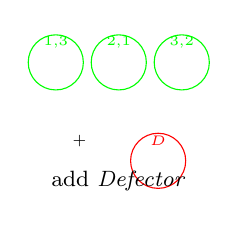
\begin{tikzpicture}
    \draw[green] (0.2, -1) circle (0.35);
    \node[green] at (0.2, -0.75) {\tiny 1,3};
    \draw[green] (1, -1) circle (0.35);
    \node[green] at (1, -0.75) {\tiny 2,1};
    \draw[green] (1.8, -1) circle (0.35);
    \node[green] at (1.8, -0.75) {\tiny 3,2};
    \node at (0.5, -2) {\tiny +};
    \draw[red] (1.5, -2.25) circle (0.35);
    \node[red] at (1.5, -2) {\tiny \(D\)};
    \node at (1, -2.5) {\footnotesize add \textit{Defector}};
\end{tikzpicture}};
    \node[roundnode](select_strat) [right=of defector] {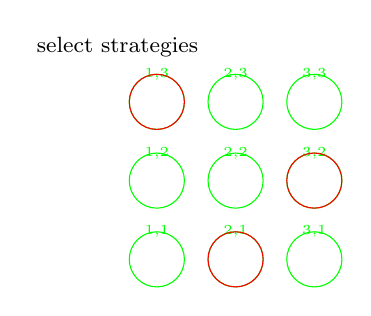
\begin{tikzpicture}
    %\draw[thin, dashed] (0, 0) rectangle (3, 3);
    \foreach \x in {1, 2, 3}
        \foreach \y in {1, 2, 3}
            {\draw[green] (\x-0.5, \y-0.5) circle (0.35);
            \node[green] at (\x-0.5, \y-0.15) {\tiny \x,\y};}
    \node at (0, 3.2) {\footnotesize select strategies};
    \draw[red] (1-0.5, 3-0.5) circle (0.35);
    \draw[red] (2-0.5, 1-0.5) circle (0.35);
    \draw[red] (3-0.5, 2-0.5) circle (0.35);
\end{tikzpicture}};
   \node[squarenode](noise&probs) [left=of defector] {FOR ALL $p_{n}$ \& $p_{e}$};
   \node[roundnode](payoffs) [below=of defector] {\begin{tikzpicture}
    \node at (-0.5, 0) {\tiny payoffs};
    \draw[->, thick] (0.5, 0) -- (0.75, 0);
    \draw[blue, dashed] (0.75, -0.25) rectangle (1, 0.25);
    \draw[blue] (1, -0.5) rectangle (2, 0.5);
    \draw[blue, dashed] (2, -0.25) rectangle (2.25, 0.25);
    \draw[->, thick] (2.25, 0) -- (2.5, 0);
    \node at (3.5, 0) {\tiny Nash eq.};
    \node at (0, 2) {\footnotesize calculating Nash eq.};
    %\node[above] at (1.75, -0.25) {\tiny support enumeration algorithm};
\end{tikzpicture}};
   \node[roundnode](tournament) [left=of payoffs] {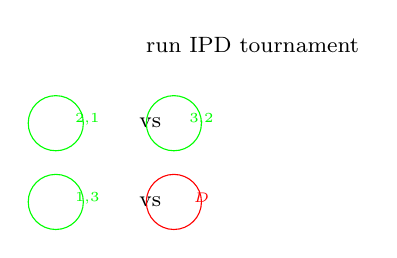
\begin{tikzpicture}
    \draw[green] (0,0) circle (0.35);
    \node[green] at (0.4, 0.05) {\tiny 2,1};
    \node[thick] at (1.2, 0) {\footnotesize vs};
    \draw[green] (1.5, 0) circle (0.35);
    \node[green] at (1.85, 0.05) {\tiny 3,2};
    \draw[green] (0, -1) circle (0.35);
    \node[green] at (0.4, -0.95) {\tiny 1,3};
    \node[thick] at (1.2, -1) {\footnotesize vs};
    \draw[red] (1.5, -1) circle (0.35);
    \node[red] at (1.85, -0.95) {\tiny \(D\)};
    \node at (2.5, 1) {\footnotesize run IPD tournament};
\end{tikzpicture}};
   \node[squarenode](writing) [right=of payoffs] {WRITE RESULTS TO DATABASE};
   \draw[->] (start.east) -- (database.west);
   \draw[->] (database.east) -- (while.west);
   \draw[->] (while.east) -- (15, 0) |- (select_strat.east);
   \draw[->] (select_strat.west) -- (defector.east);
   \draw[->] (defector.west) -- (noise&probs.east);
   \draw[->] (noise&probs.west) -- (-6, -6.12) |- (tournament.west);
   \draw[->] (tournament.east) -- (payoffs.west);
   \draw[->] (payoffs.east) -- (writing.west);
   \draw[->] (writing.east) -- (16, -13.1) |- (select_strat.east);
\end{tikzpicture}
}
    \caption{Representation of the algorithm used to collect the data.}\label{fig:alg_diag}
\end{figure}

From Figure~\ref{fig:alg_diag}, it can be seen that the first step was to set up an
empty database ready to input each tournament result into. 
The specific details of implementation into the algorithm is discussed in Section~\ref{sec:Databases}. However, the choices made on the attributes to
collect are described here. 

\begin{table}
\centering
\begin{tabular}{>{\raggedright}p{0.3\linewidth}>{\raggedright\arraybackslash}p{0.6\linewidth}}
    \toprule
    \textbf{Attribute}                   & \textbf{Description} \\
    \midrule
    experiment\_number           & A unique seed for each tournament run. \\
       
    number\_of\_players           & The number of strategies including the
    Defector. \\
             
    tournament\_player\_set       & A unique number for a particular set of
    strategies. \\
        
    player\_strategy\_name        & The strategy name as given
    in~\cite{axelrodproject}. \\
      
    is\_long\_run\_time            & Characteristic from~\cite{axelrodproject}.
    \\
          
    is\_stochastic               & Characteristic from~\cite{axelrodproject}. \\ 
       
    memory\_depth\_of\_strategy    & Characteristic from~\cite{axelrodproject}.
    \\
       
    prob\_of\_game\_ending         & The value of \(p_{e}\). \\
         
    payoff\_matrix               & A string of the matrix of mean payoff values
    from the tournament. \\
    
    num\_of\_repetitions          & A value indicating how many iterations of
    the tournament is required. \\  
          
    num\_of\_equilibria           & The number of equilibria yielded as output
    from the algorithm. \\
        
    nash\_equilibria             & A string containing the list of equilibria. \\
    
    least\_prob\_of\_defection     & The lowest probability of playing the
    \textit{Defector} obtained from the Nash equilibria. \\ 
     
    greatest\_prob\_of\_defection  & The highest probability of playing the
    \textit{Defector} obtained from the Nash equilibria. \\
    
    noise                       & Level of standard PD noise, \(p_{n}\). \\
                      
    warning\_message             & This column contained a string if the
    algorithm detected potential degeneracy. \\
    \bottomrule
\end{tabular}
\caption{Table of attributes collected.}\label{tab:attr_tab} 
\end{table}

\newpage
Table~\ref{tab:attr_tab}, shows each attribute chosen to be observed in this
study. The attributes experiment\_number and tournament\_player\_set were used
to provide a unique identification for each tournament and set of strategies.
This was to ensure clear separation during analysis. The three characteristics of the strategies
were collected with the aim of analysing the different strategies'
effect on the \(p\)-threshold. The attributes least\_prob\_of\_defection,
warning\_message, number\_of\_players and noise were the most important
attributes to this study. These were the main effects analysed with regards to the \(p\)-threshold and key descriptors of the game. The rest of the attributes
were retained: for evaluation of degeneracy; in order to replicate the
tournaments for validity; and for further research.

Following this came the choice of opponents. The number of opponents selected
ranged from one to eight and were randomly selected from the appropriate
collection of strategies in the Axelrod library~\cite{axelrodproject}. Out of
the 235 strategies currently implemented in Axelrod, only 216 were valid for
this experiment. Since this prroject was considering the Folk Theorem for the IPD,
research strategies which `cheated' (that is, those which return False when
entered into the `obey\_axelrod' function) were omitted. The \textit{Defector} strategy
was also removed as it would later be added to all sets of players. Furthermore,
due to time constraints, the 18 strategies which are classified as having a long
execution time were omitted. 

The actual IPD tournament was run using the original Axelrod tournament
setup~\cite{adeoye2012application} as implemented in the
Axelrod library~\cite{axelrodproject}. This is a round-robin type tournament where each
strategy plays every other strategy once~\cite{axelrod1980effective}.
Each round robin was repeated 500 times to obtain `smoother' estimates of
the mean payoff values. Moreover, each strategy set was run in a tournament for
100 values of \(p_{e}\) within the range \([0.001, 0.999]\). Note, zero was
not included as this implies the tournament would never end and one was
omitted as the tournament would immediately end after the first turn. However,
it is possible for the probabilities within the range \([0.999, 1]\) to be
included in this range; and this is recommended for
future research. These tournaments were also repeated for values of \(p_{n}\) in the set, \( \{0.1, 0.2, \ldots, 1\} \). The main output of interest
from each tournament is the payoff matrix, which is then implemented as the game
matrix in the Nashpy library~\cite{Nashpy2019}.
According to~\cite{axelrodproject}, each entry \(a_{i,j}\) gives the mean payoff
of player \(i\) against player \(j\). Consider the following example:
\begin{equation}
    \begin{pmatrix}
        2.990 &   2.996  &   0.487\\  
        2.996 &   3.000  &   0.989\\
        3.053 &   1.042  &   1.000        
    \end{pmatrix}
\end{equation}\label{eqn:payoff_matrix_ex}
The matrix in~\eqref{eqn:payoff_matrix_ex} is yielded from a three player
tournament with \(p_{e}=0.001 \text{ and } p_{n}=0\). The strategies in this case were \textit{Colbert}; \textit{Tideman and Chieruzzi} and
\textit{Defector}. In this case, the entry \(a_{1,2} = 2.996\) is interpreted as the
mean payoff between \textit{Colbert} and \textit{Tideman and Chieruzzi}. 

For the calculation of the Nash equilibria, the support enumeration
algorithm was used. This algorithm as well as the justification of its use is
provided in Section~\ref{sec:Calculating_Nash_Equilibria}.

Finally, the values obtained were written to the database file. One record is
inserted for each strategy in order to retain all characteristics. Here, any
entries that were not integers or floats had to be converted to strings, in order
to be stored. For example, the payoff matrix given
in~\eqref{eqn:payoff_matrix_ex} is a list and hence could not be inserted into the
database in its current format.


In summary, pseudo code for the overall algorithm is provided
in Algorithm~\ref{alg:folk_thm_explore}.

\IncMargin{2em}
\begin{algorithm}[H]
    \footnotesize
    \DontPrintSemicolon
    \SetKwInOut{Input}{input}
    \SetKwInOut{Output}{output}

    \Input{maximum number of opponents, number of strategy sets for each number
    of opponents, set of \(p_{n}\), set of \(p_{e}\), number of tournament repetitions, the
    database file path, and whether or not support
    enumeration should be used to calculate the Nash equilibria.}
    \Output{a database containing the results as detailed previously.}
    \While{True}{
        \For{each number of opponents}{
            \For{each repetition with the same number of strategies}{
                Randomly select a set of opponents and add in the \textit{Defector}.\\
                \For{each \(p_{n}\)}{
                    \For{each \(p_{e}\)}{
                        Run the IPD tournament.\\
                        Obtain the Nash equilibria and the corresponding
                        probabilities of defection, using the algorithm
                        indicated.\\
                        \For{each player in the current set}{
                            Write the required information to a record in the
                            database file.\\
                        }
                    }
                } 
            }
            Repeat
        }
    }
    \caption{Folk Theorem Exploration}\label{alg:folk_thm_explore}
\end{algorithm}
\DecMargin{2em}

\section{Databases}\label{sec:Databases}
There are many different options regarding types of file available for storage of
data. For example, csv, json, tex, txt, db extensions. These are generally split into
two types: plain text and binary files. In this section, the justification for
using an SQLite database is provided, along with how this was implemented.
However, firstly the advantages and drawbacks of plain text and binary files are
discussed.

Plain text, or flat file, is a format which stores data entries in a single table
with columns separated by delimiters such as commas or tabs~\cite{Techopedia2011}.
The contents are comprehensible by humans. Examples of these
include csv and txt extensions. The advantages of plain text formats include: a simple
structure, less disk space used and portable~\cite{Techopedia2011}. However, there
are also drawbacks. Flat files are not scalable and
are protected by less security~\cite{Thomas2018}. Only one user can edit the file at any one time
and, when wanting to search through the file, it has to be fully loaded in the
system~\cite{Burke2017}. Moreover, the columns must all contain the same data type~\cite{Techopedia2011}.

On the other hand, binary file is a format in which the sequences of zeros and ones are
unconstrained, compared to plain text files (where the binary codes have to
represent character sets)~\cite{Spacey2017}. Databases, executables and media
files are examples of these~\cite{Spacey2017}. The benefits of using binary file formats
include: uses less storage space, is less effort computationally and more
secure (it is not understood by humans)~\cite{Azad}. Although this also a
disadvantage as it makes a file harder to edit~\cite{Azad}.

\subsection{Types of Database}\label{subsec:Types_of_DB}
Using the reasons provided above, it was decided that a binary file, in
particular a database file, would be
the most appropriate format to use. Primarily, this was due to the fact that
databases are generally more robust and support out of memory operations.
Indeed, a csv file could have been used however every entry would have needed to be
a string and, if this contained commas, would break the column structure. Research into the ideal
file format for database collection resulted in the identification of two main
types of databases: relational and noSQL (Not Only SQL).

Relational databases are a file format which store data according to the
relational model described in~\cite{Codd2002}. Examples of relational
databases management systems include: SQLite, MySQL, PostgreSQL, Oracle and Db2.
Briefly, this model involves structuring the data into a table, where each
row is an observation with unique ID, or key, and each column is an
attribute. This provides an ideal way to identify relationships
between the varying records. The model was developed in the 1970s and was
motivated by the reason that, originally, structures of databases varied with the
application used. There are many advantages to a relational
database format, including: data consistency --- the data is immediately available
across several instances of the database, no `catch-up' time is needed; commitment
--- strict rules regarding permanent changes within the database;
stored procedures are allowed --- blocks of code which can be repeatedly accessed; SQL
(Structured Query Language), which has been developed for ease of query performance
using mathematics; and data
locking / concurrency --- allows many users to query the database
simultaneously without conflicts. A good paper on the model and benefits of
relational databases is~\cite{Oracle2020}. On the other hand, one major
drawback to this format is its performance in handling extremely large data
sets; which have become increasingly popular. Once the data goes beyond a
certain size, a relational database has to be distributed across many servers.
Also, this model does not support high scalability, that is, relational models
are unable to support large volumes of workloads. Furthermore, the strict structure
required for this format means that, if data cannot be easily transformed
into this structure, the complexity of the model increases. The
article~\cite{Jatana2012}, provides a more detailed description of these disadvantages. 

Alternatively, noSQL databases were created with the motivation to be more
efficient with large volumes of data. There are several different types of noSQL
databases. Key-value store databases, such as RIAK, store the data as a
simplistic key-value pair and are similar to hash tables. Column-oriented
databases, for example Cassandra, are hybrid row-column databases and
document-oriented databases, such as MongoDB, store `records' in the form of
documents with a unique key for representation. Finally, graph databases and
object-oriented databases, such as Neo4j and Db4o, respectively, store the data
as graphs (in the former case) and as objects, similar to those in Object
Oriented Programming (in the latter case). Advantages of noSQL databases
include: more flexibility with a wide range of models available; supports
scalability; and are more efficient. However, these models are relatively new in
comparison with relational models and there is no standard querying language.
Also, some of these databases are not as effective as relational databases
with regards to consistency and commitment; and maintenance is challenging. For a more
detailed approach to noSQL, see~\cite{Nayak2013}.    

Using this information, it was decided that a relational database would be the
most appropriate. Although it was intended that a large amount of data would be
collected, due to time limitations, the database was unlikely
to become too big for the system. Moreover, the structure and consistency of a
relational model was ideal for comparison of the IPD experiments. The database
management system decided upon was SQLite. This was due to the fact that there
exist Python libraries, for example SQLite3 and SQLAlchemy, for accessing the
database and its contents. Also, it is portable, with the entire database stored
in a single file, meaning it could be transferred easily from the varying
computers being used. According to~\cite{ostezer2019}, other benefits include:
its ease of use, with no configuration files, and the fact it is self-contained.

\newpage
\subsection{Implementation of the Database}
The ability to import results straight from Python was through the library
SQLAlchemy~\cite{sqlalchemy}. This allowed for the creation of the database
through to accessing the results, via Python functions and expressions.  
For example, consider the code in Listing~\ref{code:python_to_db} which was used to insert a record of
results for one strategy into the database.

\begin{listing}
\begin{minted}[frame = lines, framesep = 2mm, fontsize = \scriptsize, bgcolor = Cornsilk]{python}
    database_management_sys = sa.create_engine(
        "sqlite:///" + database_filepath + "main.db"
    )
    connect_dbms_to_db = database_management_sys.connect()

    read_into_sql = """
        INSERT into folk_theorem_experiment 
            (experiment_number, number_of_players, tournament_player_set, 
            player_strategy_name, is_long_run_time, is_stochastic, 
            memory_depth_of_strategy, prob_of_game_ending, payoff_matrix, 
            num_of_repetitions, num_of_equilibria, nash_equilibria, 
            least_prob_of_defection, greatest_prob_of_defection, noise, 
            warning_message)
        VALUES 
            (?, ?, ?, ?, ?, ?, ?, ?, ?, ?, ?, ?, ?, ?, ?, ?)
    """

    record = (
        experiment_number, number_of_players, tournament_player_set,
        str(player_strategy_name), is_long_run_time, is_stochastic,
        memory_depth_of_strategy, prob_of_game_ending, payoff_matrix_as_string,
        num_of_repetitions, num_of_equilibria, nash_equilibria_as_string,
        least_prob_of_defection, greatest_prob_of_defection, noise,
        warning_message,
    )

    connect_dbms_to_db.execute(read_into_sql, record)
\end{minted}
\caption{Python code used to record the results for a single strategy into the database.}\label{code:python_to_db}
\end{listing}

Moreover, to ensure records were being inserted into the database correctly, the
graphical user interface, DB Browser~\cite{piacentini2015db} was utilised. It is implemented
with a ``familiar spreadsheet-like interface'' for ease of use and is compatible
with SQLite databases which made it ideal for this use~\cite{piacentini2015db}.
See Figure~\ref{fig:db_browser_scrnsht}, for a screenshot of the interface.

\begin{figure}
    \centering
    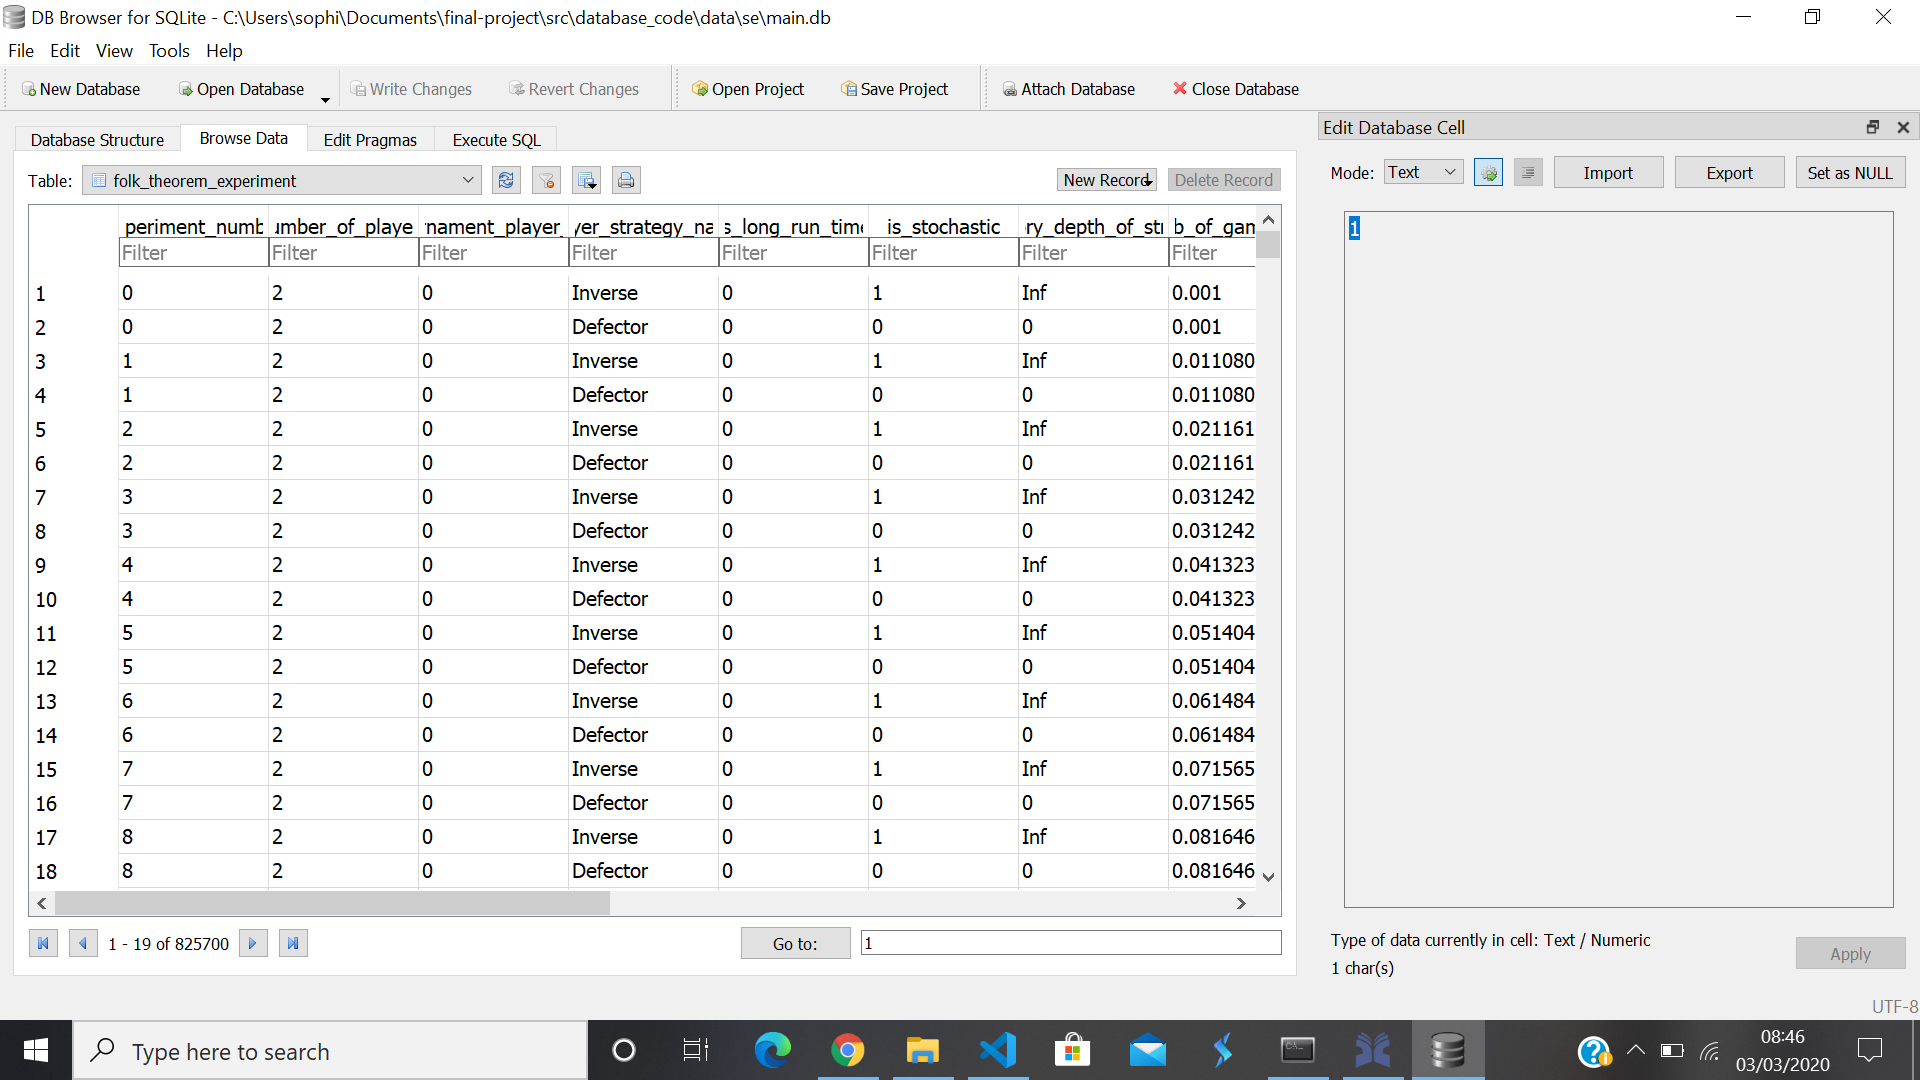
\includegraphics[width=\textwidth]{db_gui_scrnsht.png}
    \caption{DB Browser, a database graphical user interface.}\label{fig:db_browser_scrnsht}
\end{figure}


\section{Software Implementation}\label{sec:Software_Implementation}
There were many potential choices of language for the execution of this 
experiment. However, Python had the added advantage of pre-existing libraries, 
Axelrod~\cite{axelrodproject} and Nashpy~\cite{Nashpy2019}, which enabled running the IPD as well as calculation of the 
Nash equilibria. Thus, Python was used for the collection and analysis of 
data.

Throughout the implementation of this experiment into Python, good software
development principles were followed~\cite{Jimenez2017, Sandve2013, Wilson2014}. Self-documenting code was 
ensured through the careful naming of variables, as well as the use of 
docstrings to fully describe function parameters and usage. Python libraries 
Black~\cite{Langa2019} and Blackbook~\cite{Knight2019a} assisted in improving the readability of the code, through 
formatting according to the guidelines of PEP-8~\cite{Rossum2001}. This gave consistency to all 
code files created during the study. Moreover, modularity was ensured through the creation of several 
smaller functions, focusing on one task. This not only assisted with debugging,
it also allows for future usability of the code in newer developments.

Testing is another key part of software development to guarantee the durability of 
the code. Thus unit tests were implemented, using Pytest~\cite{pytestx.y}, to
assist with the 
identification of bugs in the functions created for data collection. However, 
further work in this area is needed to provide a fully tested program. 
Indeed, from executing the Python library Coverage~\cite{Batchelder2020}, a
coverage of 59\% was identified (for the `experiment\_functions.py' file), 
yielding Table~\ref{tab:cov_scrnsht}. This could be improved through the creation of 
integration tests, between the database and the experiment results, or the 
implementation of functional tests, to confirm the end result of the full 
algorithm.

\begin{table}
    \centering
    \resizebox{\textwidth}{!}{\begin{tabular}{lcccc}
    Module & statements & missing &	excluded & coverage \\
    \midrule
    src/database\_code/\_\_init\_\_.py &	0 &	0 &	0 &	100\% \\
    src/database\_code/experiment\_functions.py &	87 & 36 & 0 & 59\% \\
    src/database\_code/run-experiment-support-enumeration.py & 6 & 6 & 0 & 0\% \\
    src/database\_code/run-experiment-vertex-enumeration.py & 6 & 6 & 0 & 0\% \\
    \midrule
    Total &	99 & 48 & 0 & 52\%
\end{tabular}}
    \caption{A screenshot of the html report produced when utilising Coverage.}\label{tab:cov_scrnsht}
\end{table}

The use of version control is key for keeping track of past changes 
to the system. In this study the software Git~(https://git-scm.com/) was used. This allowed for the 
adaption of code from several different function attempts and, through GitHub~(https://github.com/), 
enabled collaboration between the author and supervisors as seen
in Figure~\ref{fig:github_scrnsht}. The use of GitHub ensured that a back-up copy
of all project files 
were available, should the current system happen to fail. Moreover, it acted as
an intermediate step between the author's laptop and the remote server, which
was used for
running the main experiment (see Section~\ref{sec:Remote_Computing}).

\begin{figure}
    \centering
    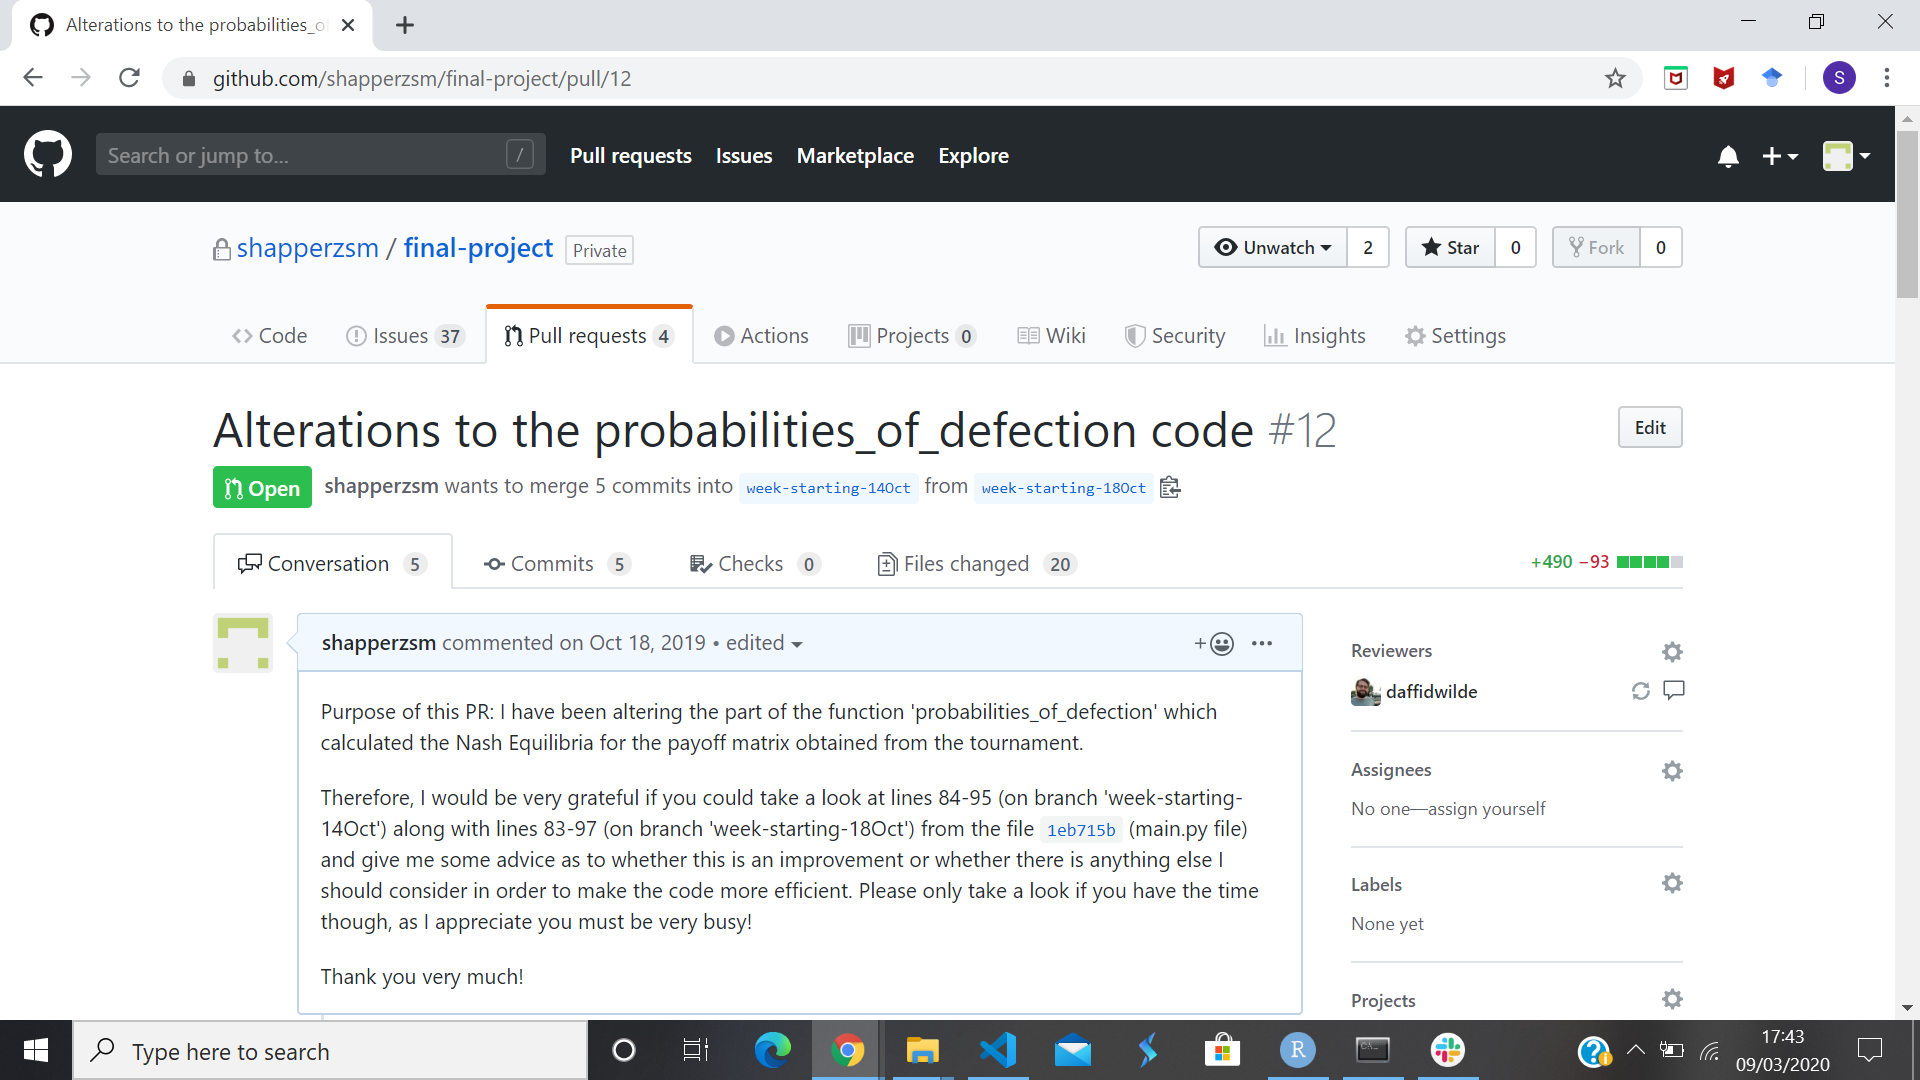
\includegraphics[width=\textwidth]{github_scrnsht.png}
    \caption{A screenshot of a GitHub pull request which allowed for collaboration between supervisors and author.}\label{fig:github_scrnsht}
\end{figure}


\section{Remote Computing}\label{sec:Remote_Computing}
This section describes the execution of the experiments via a remote
computer and the reasons for doing so.

Firstly, due to the volume of data that was planned on being collected, it was
decided that running the data remotely would be ideal, in order to allow the
code to run uninterrupted for several weeks. Thus, Cardiff University School of
Mathematics' computer Siren, a headless server with large storage, was used. However, when a trial was executed,
it was decided that the run time was `quick enough' and hence parallel
processing would not be necessary. Yet, for future runs of the code, parallel
processing is recommended, especially if the player set sizes being trialled are
`large'. See Section~\ref{subsec:Alg_Execution_Times} for an explanation.

\begin{figure}
    \centering
    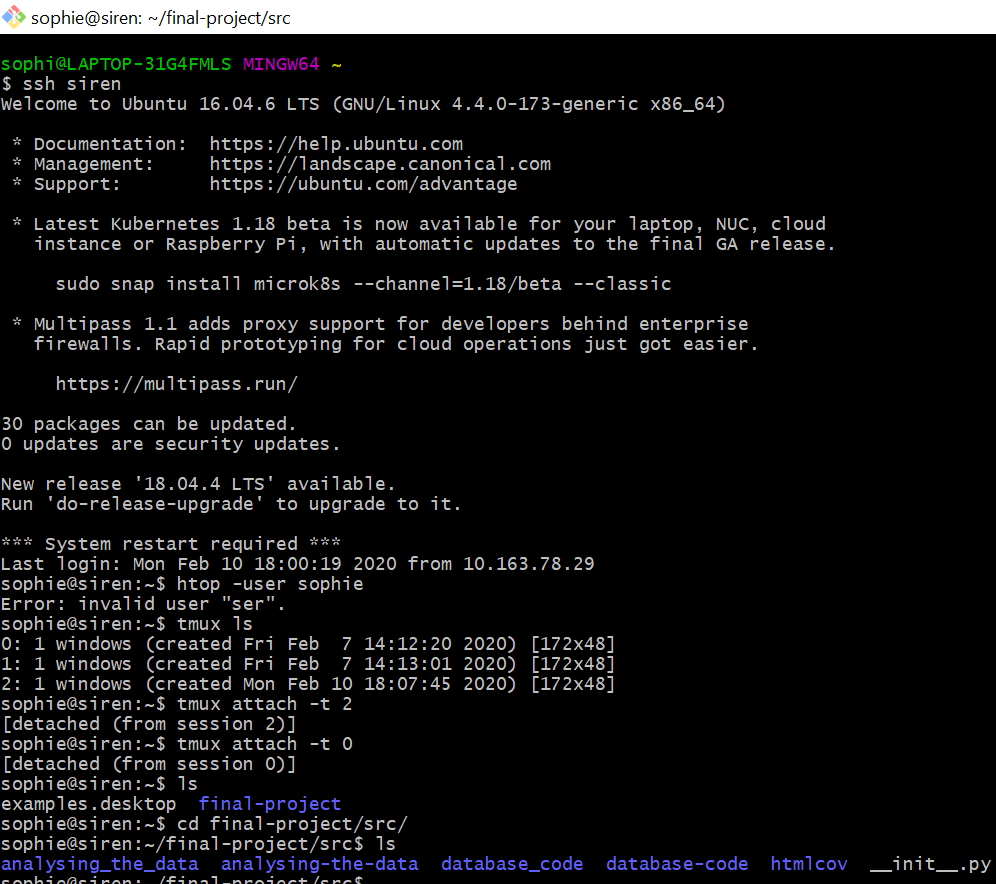
\includegraphics[width=\textwidth]{siren_scrnsht.png}
    \caption{A screenshot of the authors connection to Siren via an SSH tunnel.}\label{fig:siren_scrnsht}
\end{figure}


To connect to Siren, an SSH tunnel was used. An SSH (or Secure Shell) tunnel is
used for sending and receiving network data over an encrypted connection. It adds
a layer of network security, to those applications that do not natively support
encryption, and lowers the risk of interception. For a more detailed description
of SSH, see~\cite{SSH.COM2016}. Figure~\ref{fig:siren_scrnsht} shows the author's
connection to Siren via SSH\@. 


In order for the experiment to keep running, whilst disconnected
from Siren, a terminal emulator was required, as Siren does not have a job
scheduler. Specifically, the terminal multiplexer, TMUX~\cite{Marriott} was used. This allowed
for the creation and execution of several terminals from one screen. Moreover, a
user could detach from a terminal and reattach later without execution being
halted. Figure~\ref{fig:remote_comp}, shows a diagram of how the remote server, ssh tunnel, and user's
laptop, were all in connection.

\begin{figure}
    \centering
    % remote computing diagram
\begin{tikzpicture}
    \draw[dashed] (0,0) rectangle (14,7);
    \draw[blue, thick] (1,2.25) rectangle (4,4.25);
    \node[blue, below] at (2.5, 3.5) {\small author's laptop};
    \draw[green, thick] (8, 1) rectangle (12.5, 5.5);
    \node[green, above] at (12, 6) {\small remote server};
    \draw[orange, dashed] (10.5, 3.5) rectangle (12,5);
    \draw[orange, dashed] (8.5, 3.5) rectangle (10,5);
    \draw[orange, dashed] (10.5, 1.5) rectangle (12,3);
    \draw[orange, dashed] (8.5, 1.5) rectangle (10,3);
    \node[orange, above] at (11,1) {\small TMUX sessions};
    \draw[snake=coil, red, thick, segment aspect=0] (4.5,3.5) -- (7.5, 3.5);
    \draw[snake=coil, red, thick, segment aspect=0] (4.5,2.5) -- (7.5,2.5);
    \node[red, above] at (6, 2.75) {\small ssh tunnel};
\end{tikzpicture}
    \caption{Representation of how the experiments were run remotely. Note, `tmux sessions' correspond to emulators of terminals.}\label{fig:remote_comp}
\end{figure}

Once the experiment was running, the database had to be copied from
Siren in order for analysis to begin. This was also achieved via SSH\@. Note, the code was written in a way
which enabled the results to be written to the database concurrently, after
every tournament. This was done to ensure that, if the system were to break, data
would still have been available and retained within the database. This meant
the database file was almost always `open' resulting in the integrity check
failing once transferred over SSH and an OperationalError in SQLAlchemy. Thus, in
order to to load the database, with no failures, into a Jupyter Notebook, it
needed to be compressed before transferring. This was achieved using the command
line code as seen in Figure~\ref{fig:cmd_code_db}.

\begin{figure}
    \centering
    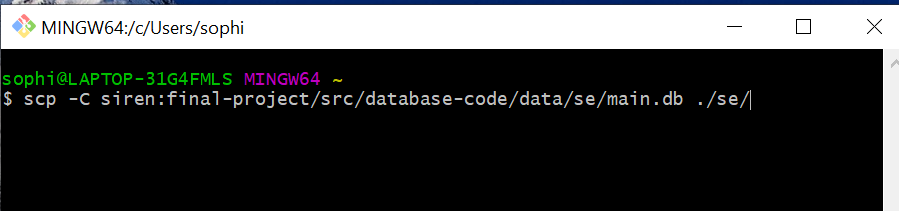
\includegraphics[width=\textwidth]{cmd_line_scrnsht.png}
    \caption{Command line code used to retrieve the database from the remote server.}\label{fig:cmd_code_db}
\end{figure}

\section{Calculating Nash Equilibria}\label{sec:Calculating_Nash_Equilibria}
Recall Nash's Theorem, Theorem~\ref{thm:Nash},
explains that there exists at least one equilibrium in every finite game.
However, it does not indicate how to obtain them. The proof of the theorem
relies on finding the fixed point of the defined mapping but the proof of
Brouwer's Fixed Point Theorem is an existence, and not a constructive, proof.
That is, it does not give a method for obtaining the fixed point. Indeed,
although not NP-complete\footnote{Both finding Brouwer fixed points and Nash
equilibria cannot be NP-complete since existence of a solution is
guaranteed~\cite{NoamNisan2007}. Most problems in the set NP-complete are situations in which
a solution might not exist~\cite{NoamNisan2007}. However,~\cite{papadimitriou1994complexity} has shown that these two
problems belong to a alternative complexity class, PPAD or Polynomial Parity
Argument (Directed case). For a discussion into this, readers are referred to~\cite{papadimitriou1994complexity}.}, finding Brouwer fixed points has been shown to be a 
hard problem~\cite{Hirsch1989,papadimitriou1994complexity}. Thus, defining algorithms which obtain Nash equilibria to
some degree of efficiency has been a large research topic for many years,
particularly in the 2000s. Example papers include~\cite{Bossea,Chen2006,Gilpina,Govindan2003,Kontogiannis2006,Krawczyk2000,Littman2005}. Within the Python Library Nashpy~\cite{axelrodproject}, three
such algorithms have been
implemented: Support Enumeration, Vertex Enumeration and Lemke-Howson. However,
the Lemke-Howson Algorithm will only find \textit{one} equilibria and hence is not
suitable for this study. Therefore the definitions of the first two algorithms,
in the case of a two player game, are provided. Unless specified otherwise, this
section (Section~\ref{sec:Calculating_Nash_Equilibria}) is adapted from~\cite{NoamNisan2007}.


\subsection{Support Enumeration}\label{subsec:Support_Enumeration}
Before stating the method for the support enumeration algorithm, a few extra
theoretical ideas are needed. 

Recall, a \textit{mixed strategy}, \(\sigma \), is a probability distribution
over the pure strategies.

\newpage
\begin{definition}
    The \emph{support} of \(\sigma \) is the set of all pure strategies, \(s_{i}
    \in \sigma \), such that \(s_{i} > 0\). That is, all pure strategies which
    have a positive probability within the mixed strategy.
\end{definition}

\begin{definition}
    A game \(G = (N, {(S_{i})}_{i \in N}, {(u_{i})}_{i \in N})\)
    is called \emph{non-degenerate} if no mixed strategy of support size \(1 \le
    k \le |S_{i}|\) has more than \(k\) pure best responses.
\end{definition}\label{def:non_degen}

For example, consider the following 2-player normal form game:
\begin{equation}
        A = \begin{pmatrix}
                2 & 1 & 0\\
                2 & 0 & 3
        \end{pmatrix}
\end{equation}\label{eqn:degen_game}


In~\eqref{eqn:degen_game}, if the column player was playing the strategy \(\sigma_{2} = (0.2, 0.8,
0)\) then the support is \{strategy1, strategy2\}. Also, observe that, if the
column player picked strategy1 then the row player could choose either their
first or second strategy and hence this game is \textit{degenerate}. 

The method of support enumeration is given in Algorithm~\ref{alg:supp_en}.

\IncMargin{2em}
\begin{algorithm}
    \footnotesize
    \DontPrintSemicolon
    \SetKwInOut{Input}{input}
    \SetKwInOut{Output}{output}

    \Input{A \emph{nondegenerate} two-player normal form game, where \(A, B\)
    are the row and column player's payoff matrices and \(\sigma_{1},
    \sigma_{2}\) are their strategy vectors, respectively.}
    \Output{Every Nash equilibrium of the input game.}
    \For{all \(k = 1, \ldots, \min{\{m, n\}}\)}{
    \For{all support pairs \(I, J\), with \(I \in M, J \in N\) and
    \(|I|=|J|=k\)}{
            Solve \begin{equation}
    \sum_{i \in I}{\sigma_{1i}B_{i,j}} = v, \text{ such that } \sum_{i \in
    I}{\sigma_{1i}} = 1, \sigma_{1i} \ge \textbf{0} \text{ for all } j \in J
            \end{equation}\label{eqn:lin_eqn_1_se} and 
            \begin{equation}
                    \sum_{j \in J}{A_{i, j}\sigma_{2j}} = u, \text{ such that }
                    \sum_{j \ in J}{\sigma_{1i}} = 1, \sigma_{1i} \ge
                    \textbf{0} \text{ for all } i \in I     
            \end{equation}\label{eqn:lin_eqn_2_se}\;
            
            Check the best response conditions \begin{equation}
                \sigma_{1i} > 0 \implies {(A\sigma_{2})}_{i} = \max \{{{(A\sigma_{2})}_{k} | k \in M}\}
            \end{equation} and 
            \begin{equation}
                \sigma_{2j} > 0 \implies {(\sigma_{1}B)}_{j} = \max \{{{(\sigma_{1}B)}_{l} | l \in N}\}
            \end{equation}

        }
    }
    \caption{Support Enumeration}\label{alg:supp_en}
\end{algorithm}
\DecMargin{2em}

Note, in Algorithm~\ref{alg:supp_en}, solutions are not guaranteed to exist for (3.3) and (3.4). In this case, the support does not yield a Nash
equilibrium. 

\subsubsection{An example}
Here the computation of Nash equilibria via support enumeration is considered
for a payoff matrix obtained from a two-player IPD tournament\footnote{Note, the \textit{Defector}'s opponent in this tournament
was stochastic player, \textit{Inverse}. Here, \(p_{e} = 0.0514, ~~ p_{n} = 0\). This game was not identified as degenerate.}. 

Consider the following normal form game:
\begin{equation}
    A = \begin{pmatrix}
        3.000 & 0.829 \\
        1.686 & 1.000 \\
    \end{pmatrix}; ~~~
    B = A^{T}
\end{equation}\label{eqn:supp_en_ex}

Firstly, take \(k = 1\), that is, looking for any pure best responses:
\begin{displaymath}
    A = \begin{pmatrix}
        \underline{3.000} & 0.829 \\
        1.686 & \underline{1.000} \\
    \end{pmatrix} ~~~ B = \begin{pmatrix}
        \underline{3.000} & 1.686 \\
        0.829 & \underline{1.000} \\
    \end{pmatrix}.
\end{displaymath}

Thus, two pairs of pure best responses are visible, giving the following two
Nash equilibria:
\begin{displaymath}
    \sigma = \left \{(1, 0), (1, 0)\right \} \text{   and   } \sigma = \left \{(0, 1), (0, 1)\right \}.
\end{displaymath}

Since this is a two-player game, the only other support that needs checking is
\(I = J = \{1, 2\} \). 

Here, (3.3) and (3.4) become,
\begin{displaymath}
    3\sigma_{r1} + 0.829\sigma_{r2} = 1.686\sigma{r1} + \sigma_{r2} ~~ \text{   and   } ~~ \\
    3\sigma_{c1} + 0.829\sigma_{c2} = 1.686\sigma{c1} + \sigma_{c2}.
\end{displaymath}

Rearranging and checking the constraint \(\sum{\sigma_{r} = 1}, ~~
\sum{\sigma_{c} = 1}\), yields 
\begin{displaymath}
    \sigma_{r1} = \sigma_{c1} = \frac{19}{165} ~~ \text{ and } ~~ \sigma_{r2} = \sigma_{c2} = \frac{146}{165}.
\end{displaymath}

Note, checking the best response condition for two players with the same number
of pure strategies is trivial~\cite{Knight2019b}. However, it is included here for completeness.
\begin{displaymath}
    A\sigma_{c}^{T} = \begin{pmatrix}
        3 & 0.829 \\
        1.686 & 1 \\
    \end{pmatrix} \begin{pmatrix}
        \frac{19}{165} \\
        \frac{146}{165} \\
    \end{pmatrix} = \begin{pmatrix}
        1.079 \\
        1.079 \\
    \end{pmatrix} \text{   and   }
\end{displaymath}

\begin{displaymath}
    \sigma_{r}B = \begin{pmatrix}
        \frac{19}{165} & \frac{146}{165} \\
    \end{pmatrix} \begin{pmatrix}
        3 & 1.686 \\
        0.829 & 1 \\
    \end{pmatrix} = \begin{pmatrix}
        1.079 & 1.079
    \end{pmatrix}
\end{displaymath}

Therefore, the best response condition holds for both players. Hence, the third and final Nash equilibrium is given by:
\begin{displaymath}
    \sigma = \left \{ (\frac{19}{165}, \frac{146}{165}), (\frac{19}{165}, \frac{146}{165})\right \}.
\end{displaymath}


\subsubsection{Advantages and Drawbacks}\label{subsubsec:Adv_and_Drawbacks}
Support enumeration is known to be a robust method for obtaining Nash
equilibria. That is, given a non-degenerate game,
it is guaranteed to return all equilibria and, even in the case of degeneracy,
it will find some equilibria (see Section~\ref{sec:Degeneracy}). However, this method essentially
compares all pairs of supports and thus has an exponential complexity~\cite{Rampersaud2014}. This implies that support enumeration is
computationally expensive and the larger the game, the slower it will become.


\subsection{Vertex Enumeration}\label{subsec:Vertex_Enumeration}
Vertex enumeration is based on a geometric representation of games and hence,
in this section, a brief introduction to this is provided. The reader is
referred to~\cite{NoamNisan2007} for a more detailed approach to this topic.

\begin{definition}
    Let \(A, B\) be \emph{positive} payoff matrices for the row and column
    player; that is, each element \(a_{ij}, b_{ij} > 0\), for all \(i = 1,
    \ldots, M, j = 1, \ldots, N\). Then the row, column
    \textit{best response polytopes}\footnote{In general, a
    \emph{polytope} is defined as a bounded set \( \{z \in \mathbb{R}^{d} |
    Cz^{T} \le q\} \) where \(C\) is a \(k \times d\) matrix and \(z\) is a \(1
    \times d\) vector~\cite{NoamNisan2007}.}, denoted \(P, Q\) are given respectively by
    \begin{equation}
        P = \{x \in \mathbb{R}^{M} | x \ge \textbf{0}, ~ xB \le \textbf{1}\} ~~~
        Q = \{y \in \mathbb{R}^{N} | Ay^{T} \le \textbf{1}, ~ y \ge \textbf{0}\}.
    \end{equation}
    It is assumed that the utility values which appear
    in (3.3) and (3.4) have been normalised
    to 1. This means that the vertices are no longer probabilities and hence
    scaling will be required to find the Nash equilibria. Note, the strictly
    positive payoffs is not a constraint since a constant can be added to each
    with no effect. 
\end{definition}\label{def:best_resp_polytopes}


For example, consider the payoff matrix 

\begin{equation}
    A = \begin{pmatrix}
        1 & 5 \\
        4 & 1
    \end{pmatrix}
\end{equation}\label{eqn:ex_vert_en}

Then the best response polytope, \(P\) here is given by the inequalities:
\begin{center}
    \(
        x_{1} \ge 0, ~~
        x_{2} \ge 0, ~~
        x_{1} + 5x_{2} \le 1, ~~
        4x_{1} + x_{2} \le 1
    \)
\end{center}

which yields the following polytope as given in Figure~\ref{fig:best_resp_polytope}.

\begin{figure}
    \centering
    % best response polytope example
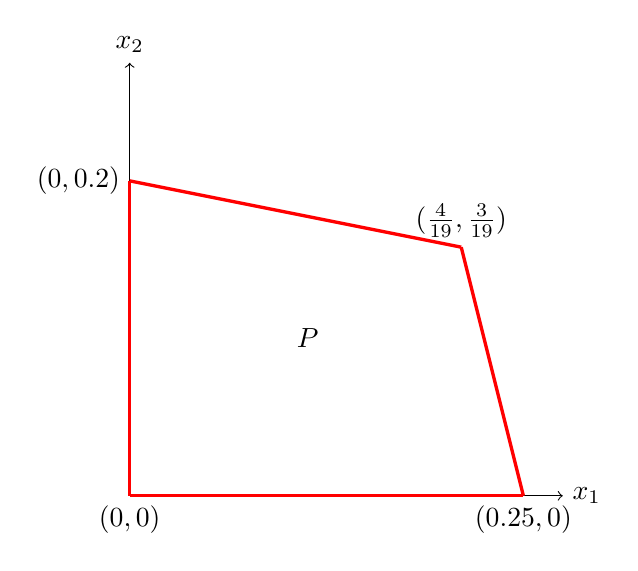
\begin{tikzpicture}
    \draw[->] (0,0) -- (5.5,0) node[right]{$x_{1}$};
    \draw[->] (0,0) -- (0,5.5) node[above]{$x_{2}$};
    \draw[red, very thick] (0,0) -- (5,0);
    \draw[red, very thick] (5,0) -- (80/19,60/19);
    \draw[red, very thick] (0,0) -- (0,4);
    \draw[red, very thick] (80/19,60/19) -- (0,4);
    \node[below] at (0,0) {$(0,0)$};
    \node[below] at (5,0) {$(0.25,0)$};
    \node[left] at (0,4) {$(0,0.2)$};
    \node[above] at (80/19,60/19) {$(\frac{4}{19}, \frac{3}{19})$};
    \node[right] at (2,2) {$P$};
\end{tikzpicture}
    \caption{Best response polytope, \(P\), obtained from the payoff matrix given in~\eqref{eqn:ex_vert_en}.}\label{fig:best_resp_polytope}
\end{figure}

Two algorithms are given, Algorithm~\ref{alg:vertex_lab} `prepares' the polytope
for Algorithm~\ref{alg:vertex_en} which returns the Nash equilibria.

\IncMargin{2em}
\begin{algorithm}
    \footnotesize
    \DontPrintSemicolon
    \SetKwInOut{Input}{input}
    \SetKwInOut{Output}{output}

    \Input{A polytope, \(P \in \mathbb{R}^{n}\).}
    \Output{A labelled-vertex polytope.}
    enumerate each of the defining inequalities of \(P\), \(c_{1}, \ldots,
    c_{k}\) \\
    \For{each vertex \(v_{i} \in P\)}{
        find the inequalities of \(P\) which are \textit{binding} at
        \(v_{i}\), that is the defining equations are equalities.\\

    the label of \(v_{i}\) is given by \( \{c_{i1}, \ldots, c_{il}\} \), where
        \(c_{ij}\) is in the label if and only if equation \(c_{j}\) is binding
        for \(v_{i}\).
    }
    \caption{Vertex Labelling}\label{alg:vertex_lab}
\end{algorithm}
\DecMargin{2em}

A pair of labels \(v_{i} \in P, ~ u_{j} \in Q\) are called \emph{fully labelled}
if every inequality `number' of \(P \cup Q\) appears in either the label of
\(v_{i}\) or the label of \(u_{j}\). Then there is a notion which states that
each fully labelled pair, when normalised, corresponds to a Nash equilibrium.
Note, this does not include the vertex pair \((\textbf{0}, \textbf{0})\) since,
although this is a fully labelled pair, it corresponds to neither opponent playing any strategies. 

\IncMargin{2em}
\begin{algorithm}
    \footnotesize
    \DontPrintSemicolon
    \SetKwInOut{Input}{input}
    \SetKwInOut{Output}{output}

    \Input{Best response polytopes, \(P, Q\), as defined
    in~\ref{def:best_resp_polytopes}, for a \emph{nondegenerate} game.}
    \Output{All Nash equilibria of the corresponding game.}
    \For{each polytope, \(P, Q\)}{
        Execute Algorithm~\ref{alg:vertex_lab}.\\
    \For{each pair of vertices \( \{u_{i}, v_{j}\} \) in \(P, Q\) respectively,
    \textit{except} \((\textbf{0}, \textbf{0})\)}{
        check if they are fully labelled.\\
        \If{they are fully labelled}{
            add to the list of equilibria.
        }\Else{
            continue
        }
    }
    }
    \caption{Vertex Enumeration}\label{alg:vertex_en}
\end{algorithm}
\DecMargin{2em}

\subsubsection{Advantages and Drawbacks}\label{subsubsec:Adv_and_Drawbacks}
Vertex enumeration is more efficient than support enumeration, according
to~\cite{NoamNisan2007}, since there are more supports in a game than there are
vertices. Indeed, consider the example of \(M = N\) where \(M, N\) are the
number of binding inequalities in the best response polytopes, \(P, Q\),
respectively. Using the support enumeration algorithm, approximately \(4^{n}\)
support pairs will need to be observed but, according to the `Upper Bound
Theorem' for polytopes~\cite{Alon1985,Brondsted2012,Seidel1995}, \(P\) and \(Q\) have less than \(2.6^{n}\) vertices.
Thus, given there exists an efficient method for enumerating vertices, this
implies less further computational complexity. However, if the game is
degenerate, this algorithm may not return any Nash equilibria. 

\subsection{Algorithm Execution Timings}\label{subsec:Alg_Execution_Times}
Due to the robustness of the support enumeration, it was decided that this would
be the main method of calculating Nash equilibria. Having said this, timings for
each of the two algorithms were obtained, to see
if their computational times were significantly different. For
the purposes of this trial run, the following parameters were used: 100
tournament repetitions, \(p_{e} = 0.2\) and \(p_{n} = 0\). The results can be
seen in Figure~\ref{fig:timing_exp}.

\begin{figure}
    \centering
    \begin{subfigure}{0.45\textwidth}
        \centering
        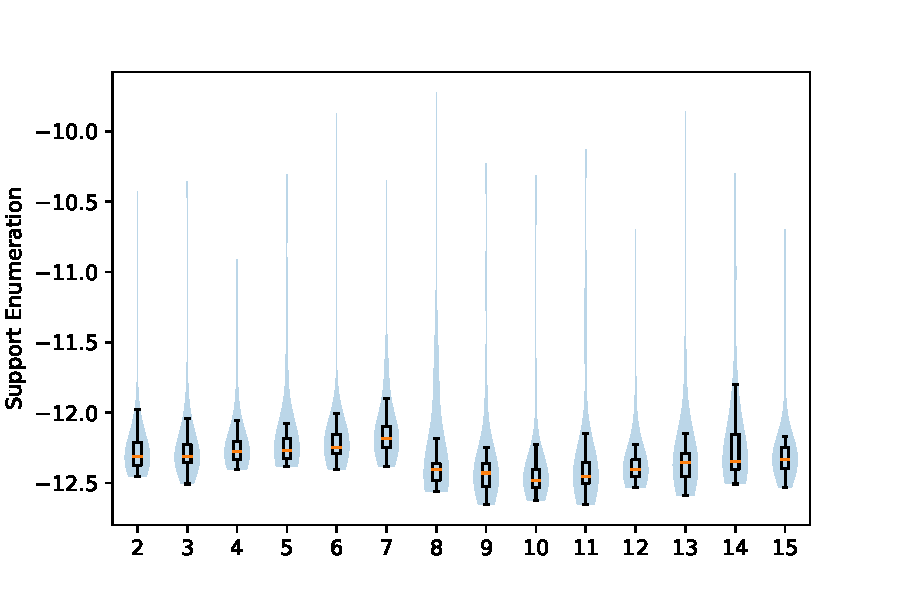
\includegraphics[width=\textwidth]{folk_thm/se_data_time_violinplot.pdf}
        \caption{Timing the support enumeration algorithm.}
    \end{subfigure}
    \hspace{3pt}
    \begin{subfigure}{0.45\textwidth}
        \centering
        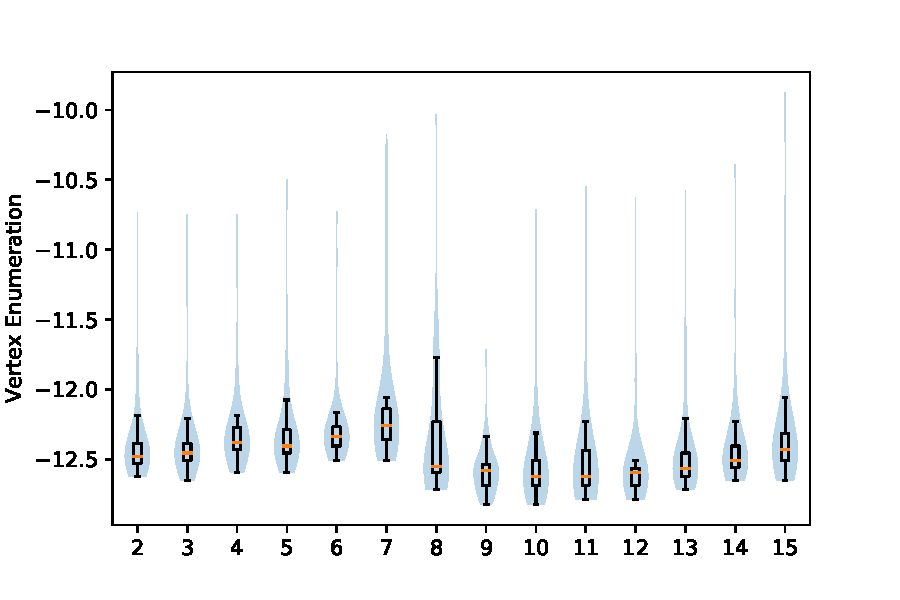
\includegraphics[width=\textwidth]{folk_thm/ve_data_time_violinplot.pdf}
        \caption{Timing the vertex enumeration algorithm.}
    \end{subfigure}
    \caption{Violinplots of the log timings obtained for the experiment and calculation of Nash equilibria using the two algorithms discussed.}\label{fig:timing_exp}
\end{figure}

From Figure~\ref{fig:timing_exp}, it can be seen that there is not a significant
difference in the execution times of the algorithms. Hence, although support
enumeration has a greater computational complexity than vertex enumeration, it
is not going to have any recognisable impact on the number of experiments
executed.


\section{Degeneracy}\label{sec:Degeneracy}
Recall, the definition of non-degeneracy, given in
Definition~\ref{def:non_degen}. This implies a \textit{degenerate} game is one in
which there exists a support of size \(k\) where the number of pure best
responses is greater than \(k\). For example, consider the following payoff
matrix:
\begin{equation}
    A = \begin{pmatrix}
        1 & 4 & 3\\
        0 & 4 & 2
    \end{pmatrix}
\end{equation}
Then, if the column players picks their second strategy (support of size 1),
the row player can pick either of their strategies (that is, two pure best
responses). Thus, this game is degenerate.

Let \(G = (N, {(S_{i})}_{i \in N}, {(u_{i})}_{i \in N})\) be a degenerate game.
Then, recall that support enumeration may not return all Nash equilibria. This
is due to the fact that if solutions to (3.3) and (3.4) of Algorithm~\ref{alg:supp_en} exist, they may not be unique. Indeed, the number of
Nash equilibria in a degenerate game may be infinite~\cite{NoamNisan2007}.
Considering degeneracy in terms of vertex enumeration implies that a vertex of
the best response polytope \(P = \{x \in \mathbb{R}^{M} | x \ge \textbf{0}, ~ xB
\le \textbf{1}\} \) may have more than \(M\) labels leading to a `badly defined'
polytope.

Within the library Nashpy, the algorithms have been implemented such that if
potential degeneracy is identified, for example, by the reasons given above, then
a warning is issued. Thus, in order to retain whether a game is possibly
degenerate, the algorithm was required to `catch' the given warnings. This
was achieved using the code seen in Listing~\ref{ls:warn_code}, with the Python
warnings module.

\begin{listing}
    \begin{minted}[frame = lines, framesep = 2mm, fontsize = \scriptsize, bgcolor = Cornsilk]{python}
    
    with warnings.catch_warnings(record=True) as w:
        warnings.simplefilter("always")

        if support_enumeration is True:
            nash_equilibria = list(game.support_enumeration())

        else:
            highlight_numpy_warning = np.seterr(all="warn")
            nash_equilibria = list(game.vertex_enumeration())

    if len(w) == 0:
        warning_message = None

    else:
        warning_message = str([w[i].message for i in range(len(w))])

    \end{minted}
    \caption{Python code used to `catch' potential degeneracy.}\label{ls:warn_code}
\end{listing}

Note, warnings for potential degeneracy are only highlighted if the
Nash equilibria obtained do not make sense, that is, are not a probability
distribution. On the other hand, it is possible for the algorithm to obtain some
correct Nash equilibria, even if the game is degenerate. This means that, any results, regarding degeneracy of the games, obtained during the
experiment (see Chapter~\ref{ch:Analysis}) need to be inferred with caution. These
are only the games caught by the algorithms in Nashpy and are not necessarily
all of them.

\section{Conclusion}
In this chapter, the creation and execution of the large experiment was
detailed in its entirety. Justifications were given as to why certain methods
and software were used or not. Also, how the Nash equilibria are calculated was
explained, with an example given. Moreover, the potential problems which could
be faced as a result of degeneracy are highlighted.